% Appendix blocks removed from the submission supplement in W100aw (appendix slimming, PI ruling 2026-10-05 item 5).
% Each block is verbatim, with its src comments; NOT \input anywhere. Values remain in the cited analysis outputs and the research record.

% ======================================================================
% FROM: sections/appendix_consequences.tex (block starting '\subsection{Paired comparisons and interval families}', 18 lines)
% WHY: G-H Holm family, Figure f9 (fig:modes) and the Qwen3-14B BFCL G-H/F-G paragraph: old Result-2 mode-ranking analysis; the main text no longer states or cites it (it cites app:r2main only for the pooled G, H, F, which Table tab:ghf and the generated new-task table carry).
% ======================================================================
\subsection{Paired comparisons and interval families}
\label{app:r2main}
\begin{figure}[t]
\centering
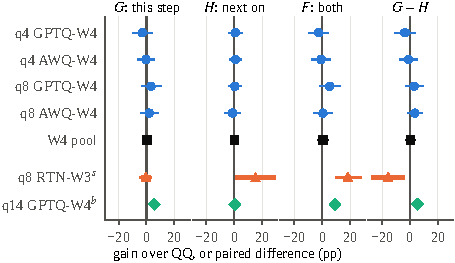
\includegraphics[width=\columnwidth]{figures/f9_upgrade_modes.pdf}
\caption{Upgrade modes on the same divergent states (\tautwo{} development; four core W4 cells and their pool). (a)~Replace this step ($G$), take over from the next step ($H$), or both ($F$), as gain in success over QQ, and the paired difference $G-H$; pp; unadjusted, thick: fixed-pool 95\%, thin: new-task 95\%, except for the cells' $G-H$ (the Holm family), where thin is the simultaneous interval and only filled markers are significant after Holm adjustment. (b)~Joint rescue (only BB succeeds) and rescue undone ($\YY{BQ}=1$, $\YY{QQ}=0$, $\YY{BB}=0$), \% of divergent states (exploratory, post hoc); thick: fixed-pool 95\%, thin: new-task 95\%. Each is a rescue that one single-mode evaluation misses. Interval details: below.} % src: analysis/fork/out/ghf_20261001T211519Z.json; analysis/fork/out/ghf_multiplicity_20261001T225727Z.md (Bonferroni 98.75%); analysis/fork/out/outcome_classes_20261004T143614Z.json
\label{fig:modes}
\end{figure}

\paragraph{Paired comparisons distinguish upgrade modes.} All three upgrade modes are measured on the same states, so they can be compared by paired differences (Figure~\ref{fig:modes}a). Over the four core W4 cells, $G-H$ is a fixed Holm family ($m=4$; fixed task pool, $t$ over blocks). In both Qwen3-8B cells, action replacement outperforms continuation takeover: $G-H=+2.9$ (GPTQ-W4) and $+3.4$\pp{} (AWQ-style W4), Holm-adjusted $p=.013$ and $.012$; this ranks the two modes and does not show that replacing the action beats QQ. In the Qwen3-4B cells the point estimates favour continuation takeover ($-3.6$ and $-1.3$\pp{}), but neither is significant after Holm adjustment. All four new-task intervals include zero, so the finding is limited to the fixed task pool and stays exploratory (intervals and further cautions below). % src: analysis/fork/out/ghf_multiplicity_20261001T225727Z.md; analysis/fork/out/ghf_20261001T211519Z.md (§1)
In the low-success stress cell q8 RTN-W3, continuation takeover beats action replacement ($G-H=-15.7$ [$-27.5$, $-3.9$]\pp{}, three blocks). % src: analysis/fork/out/ghf_20261001T211519Z.md (§1, q8:rtn_w3 row)
For Qwen3-14B GPTQ-W4 on BFCL (one exploratory configuration), action replacement wins ($G-H=+5.3$ [$+2.3$, $+8.4$]\pp{}), and action and continuation are complementary there (below). % src: analysis/fork/out/ext_q14_20261002T085647Z.md (§2, bfcl:q14:gptq_w4_d1)
The joint upgrade $F$ has the largest point estimate in both examples, and we compare no compute costs, so no cost-optimal mode is established.

\paragraph{The $G-H$ family and Figure~\ref{fig:modes}a.} In Figure~\ref{fig:modes}a, $G$, $H$, $F$ and the pool show fixed-pool 95\% (thick; block bootstrap) and new-task 95\% (thin; crossed) intervals, none multiplicity-adjusted. For the four cells' $G-H$, which form the Holm family ($m=4$), thick is the plain 95\% $t$ interval and thin the Bonferroni simultaneous 98.75\% interval; filled markers are significant after Holm adjustment, open markers are not. Above, the stress cell's $G-H$ has a $t$ interval over three blocks, and the BFCL configuration's an item-bootstrap 95\% interval; neither is drawn. % src: analysis/fork/out/ghf_20261001T211519Z.json; analysis/fork/out/ext_q14_20261002T085647Z.json; analysis/fork/out/ghf_multiplicity_20261001T225727Z.md (Bonferroni 98.75%)
The plain 95\% $t$ intervals are [$+1.0$, $+4.8$] (q8 GPTQ-W4, $G-H=+2.9$, Holm-adjusted $p=.013$) and [$+1.3$, $+5.5$] (q8 AWQ-style W4, $+3.4$, $p=.012$). In q4 GPTQ-W4 ($-3.6$) the plain interval [$-6.9$, $-0.3$] excludes zero, but the Holm-adjusted $p=.069$; q4 AWQ-style W4 ($-1.3$) has $p=.199$. Two further cautions apply. A significant result in one model and a non-significant one in the other is not a significant difference between models, and the cells select different divergent states. $G-H>0$ shows that replacing the action beats handing over the continuation, not that replacing the action beats QQ. % src: analysis/fork/out/ghf_multiplicity_20261001T225727Z.md; analysis/fork/out/ghf_20261001T211519Z.md (§1)

\paragraph{Supplementary configuration.} For Qwen3-14B GPTQ-W4 on BFCL (one configuration, one run per item, 471 divergent items; exploratory), action and continuation are complementary: keeping Q's action, a BF16 continuation adds $H=+0.4$ [$-1.1$, $+1.9$]\pp{}; after B's action has replaced Q's, the BF16 continuation adds a further $F-G=+3.4$ [$+1.3$, $+5.6$]\pp{}. % src: analysis/fork/out/ext_q14_20261002T085647Z.md (§2, bfcl:q14:gptq_w4_d1 H and F−G)

% ======================================================================
% FROM: sections/appendix_consequences.tex (block starting '\paragraph{BF16 and Q$'$ protocols.}', 2 lines)
% WHY: Pattern-frequency difference between the BF16 and Q' selection protocols: not used by the main text; the common-state comparison (app:commonstate) is the direct test it defers to.
% ======================================================================
\paragraph{BF16 and Q$'$ protocols.} On the 1020 paired task$\times$block units of the same-precision fork, the BF16 design detects a joint rescue on 3.92\% of units and the Q$'$ design on 1.76\%, a paired difference of $+2.16$\pp{} ($t$ [$+0.34$, $+3.97$]; crossed [$-0.20$, $+4.71$]); for rescue undone the difference is $-1.47$ ($t$ [$-2.97$, $+0.03$]; crossed [$-3.83$, $+0.78$]). Each design forks at its own first divergence, so these are differences in how often two selection-and-replacement protocols find the patterns, not precision effects at a common state; the common-state comparison (Appendix~\ref{app:sameprec}) is the direct test of BF16's extra action value. % src: analysis/fork/out/bf16_vs_qprime_20261005T134743Z.md (TL;DR; pool q4+q8)


% ======================================================================
% FROM: sections/appendix_consequences.tex (block starting '\paragraph{Mistral.} On Mistral', 2 lines)
% WHY: Mistral named-pattern paragraph: duplicates the Mistral row and footnote of Table tab:patternref.
% ======================================================================
\paragraph{Mistral.} On Mistral-Small-3.2-24B's own BF16-trajectory states (Appendix~\ref{app:mistral}; 464 states with differing actions, GPTQ-W4 and RTN-W4 pooled, five blocks), joint rescue is 3.4\% against a reference of 2.9\% and rescue undone 4.0\% against 4.7\%; neither difference is resolved. There BB is the recorded BF16 original rather than an upgrade of Q's state, so the denominators and the reading of the named patterns differ from Bank P, and we do not compare the two populations. % src: analysis/fork/out/mistral_patterns_20261005T135040Z.md (TL;DR; §4; §5)


% ======================================================================
% FROM: sections/appendix_consequences.tex (block starting 'On the 85 development tasks, the top 20\% of tasks account', 2 lines)
% WHY: Older concentration analysis (consequence_v2 / w67 audit): superseded by the hash-split fragility analysis of Table tab:fragility that the main-text pointer relies on.
% ======================================================================
On the 85 development tasks, the top 20\% of tasks account for 57--71\% of flips in the W4 and KV8 cells. Splitting the 20 blocks into disjoint nonce halves reproduces task-level turnover rankings (Spearman 0.52--0.86). Conditional tests control measured baseline success and, in a post-hoc variant, trajectory length; the association is carried primarily by retail and weakens on airline alone. These are retrospective associations on the same tasks under fresh prompt perturbations, rather than evidence of transfer to new tasks. % src: analysis/fork/out/consequence_v2_20261001T070850Z.json (share_of_consequences_in_top20pct_tasks); analysis/fork/out/w67_audit_v2_20261001T0600Z_20261001T070500Z.md (Concentration; panel85, airline27)


% ======================================================================
% FROM: sections/appendix_consequences.tex (block starting '\paragraph{Why a fallback cannot be judged by its average ga', 1 lines)
% WHY: Post hoc outcome-conditioned decomposition of the W4 pool net: no main-text statement relies on it.
% ======================================================================
\paragraph{Why a fallback cannot be judged by its average gain.} A post hoc decomposition of the \tautwo{} W4 pool accounts for the small net: where QQ fails (non-divergent units count as no rescue), B's action rescues 14.6\% of units, and where QQ succeeds it damages 26.1\%, but QQ succeeds in only $34.6\%$. It conditions on outcomes, so it cannot guide escalation online. % src: analysis/fork/out/task_fragility_20261005T134836Z.md (Conditional rates, pool)

% ======================================================================
% FROM: sections/appendix_confirmation.tex (block starting '\paragraph{Post-hoc four-branch estimands on the holdout.}', 21 lines)
% WHY: Post hoc four-branch estimands on the holdout (tab:holdoutr2): not part of the pre-registered confirmation and not cited by the main text; its telecom-development sentence duplicates app:holdoutdev.
% ======================================================================
\paragraph{Post-hoc four-branch estimands on the holdout.} Table~\ref{tab:holdoutr2} is a supplementary, descriptive output computed after the confirmatory analysis, with the same admission and units. It is not part of the pre-registered confirmation and changes neither the primary endpoint nor its reading. Its $G$ is a ratio over divergent states, whereas $\Gall$ in Table~\ref{tab:holdout} averages over all admitted units with non-divergent units counted as 0. % src: analysis/fork/out/holdout_r2_posthoc_20261002T024414Z.md

In a post hoc four-branch analysis of the holdout's divergent states, the pooled $H$ and $F$ are also negative ($-2.8$ and $-2.5$\pp{}), but both crossed 95\% intervals include zero, and q4 GPTQ-W4 has positive point estimates (Appendix Table~\ref{tab:holdoutr2}). The holdout changes domain as well as tasks; on the 80 telecom development tasks the same q8 configurations give $+2.7$ and $-0.6$\pp{} (Appendix~\ref{app:holdoutdev}). % src: analysis/fork/out/holdout_r2_posthoc_20261002T024414Z.md (§1 crossed 95%); analysis/fork/out/dev_all_20261001T093944Z.md (Telecom development)

\begin{table*}[t]
\centering\scriptsize\setlength{\tabcolsep}{3pt}
% src: analysis/fork/out/holdout_r2_posthoc_20261002T024414Z.md (§1 crossed 95%; §3 table and control)
\resizebox{\textwidth}{!}{\begin{tabular}{@{}lrlllllr@{}}
\toprule
Cell (weight) & states & $G$ & $H$ & $F$ & $G-H$ & mean $I$ & off-diag.\ \% \\
\midrule
q4 GPTQ-W4 (1/2) & 385 & $-3.1$ [$-9.0$, $+2.8$] & $+0.5$ [$-5.4$, $+6.4$] & $+1.8$ [$-4.8$, $+8.4$] & $-3.6$ [$-9.1$, $+1.8$] & $-4.4$ [$-12.5$, $+3.7$] & 19.7 \\
q8 GPTQ-W4 (1/4) & 399 & $-5.8$ [$-10.2$, $-1.3$] & $-4.0$ [$-10.2$, $+2.2$] & $-5.3$ [$-11.6$, $+1.1$] & $-1.8$ [$-6.4$, $+2.9$] & $-4.5$ [$-10.4$, $+1.4$] & 19.5 \\
q8 AWQ-style W4 (1/4)  & 396 & $-6.6$ [$-13.0$, $-0.1$] & $-8.3$ [$-15.3$, $-1.3$] & $-8.3$ [$-15.5$, $-1.2$] & $+1.8$ [$-3.3$, $+6.8$] & $-6.6$ [$-14.5$, $+1.4$] & 23.7 \\
\midrule
Weighted pool & 1180 & $-4.6$ [$-7.8$, $-1.5$] & $-2.8$ [$-6.3$, $+0.6$] & $-2.5$ [$-6.2$, $+1.3$] & $-1.8$ [$-4.8$, $+1.1$] & $-5.0$ [$-9.6$, $-0.4$] & 20.7 \\
\bottomrule
\end{tabular}}
\caption{Telecom holdout, \emph{post-hoc} four-branch estimands on divergent states (descriptive; not part of the pre-registered confirmation). pp; crossed task$\times$block 95\% intervals; pool weights as pre-registered; mean $I$ as in Table~\ref{tab:ghf}.}
\label{tab:holdoutr2}
\end{table*}

% ======================================================================
% FROM: sections/appendix_precision.tex (block starting '\paragraph{Overlap details (W4).}', 3 lines)
% WHY: Duplicate of the next paragraph (107 shared units, shuffle reference 76 [69, 84]); its continuation-side kappa sentence is kept, merged into that paragraph.
% ======================================================================
\paragraph{Overlap details (W4).} The two action-replacement flip sets share 107 units, against 76 [69, 84] under a within-task block shuffle that preserves task-level flip propensity. % src: analysis/fork/out/sameprec_overlap_20261002T143218Z.md (Overlap table; Agreement)
When B also takes over the continuation, rescue sets under the continuation-only contrast agree with $\kappa=0.20$, and 70\% of continuation-dependent units are continuation-dependent under one substitution only. % src: analysis/fork/out/sameprec_split_20261002T145148Z.md (Figure-panel table; §1; §2; §3)


% ======================================================================
% FROM: sections/appendix_fidelity.tex (block starting '\paragraph{KL tracks action divergence and turnover, not net', 1 lines)
% WHY: Long lead paragraph whose correlations repeat 'Across and within configurations'; replaced by a compact lead that keeps the D_cc definition, the configuration caveat and the SpinQuant/QuaRot contrast.
% ======================================================================
\paragraph{KL tracks action divergence and turnover, not net value.} On ordinary BF16-sourced states shared by every method (U2B), we compare methods by $D_{cc}=\YY{QB}-\YY{BB}$, Q's action against B's under the shared BF16 continuation, with turnover $M_{cc}$ (Appendix~\ref{app:panels}). These comparisons evaluate complete quantization configurations, including their calibration pipelines, rather than isolated algorithmic components. Across the eleven q8 configurations (descriptive Spearman), mean teacher-forced approximate token KL$(\mathrm{B}\|\mathrm{Q})$ is strongly associated with the action-difference rate ($\rho=0.99$) and with turnover ($\rho=0.925$ with $M_{cc}$). Conditional on the actions differing, its association with consequences is weak: $\rho=0.46$ with the flip rate given a difference, and within configurations a mean AUC of 0.46 for flips among differing actions, against 0.93 for separating differing from identical actions. It gives no reliable prediction of net value ($\rho=-0.44$ with $D_{cc}$), consistent with KL measuring the size of a disagreement rather than its direction \citep{nikolic2026displacement}. SpinQuant-W4A4 has lower KL than QuaRot-W4A4 (0.165 against 0.199), yet their pre-registered task-value contrast is unresolved ($+1.2$\pp{}, crossed [$-4.7$, $+7.1$]; Appendix~\ref{app:panels}). % src: analysis/fork/out/kl_decomp_20261005T000559Z.md (TL;DR; §2; §3); analysis/fork/out/newmethod_q8_20261004T051538Z.md; analysis/fork/out/newmethod_q8_20261004T051538Z.json (tau2.contrasts; fidelity.cells.*.KLu_mean); docs/insights/NEWMETHOD_PANEL_PROTOCOL.md (§2.1, §4, A1.2, A7); analysis/fork/out/backfill_20261003T193042Z.md (TL;DR 2; §2)

% ======================================================================
% FROM: sections/appendix_scope.tex (block starting '\paragraph{Ordinary states and the user simulator.} At ordin', 2 lines)
% WHY: Summary paragraph that repeats the next paragraph and the simulator control below.
% ======================================================================
\paragraph{Ordinary states and the user simulator.} At ordinary (Bank U) states, turnover is lower (W4 configurations, U1 and U2B: 4.7--9.0\%) and the net gain covers zero. Most outcome changes there come from differences in text. We could not confirm their labels under a second user simulator (one control exposed replies to sibling arms; see below), so we do not report them as a property of the action. % src: analysis/fork/out/bank_u_f01_f02_f03_20261002T003037Z.md (§2); analysis/fork/out/simctrl_20261001T212742Z.md


% ======================================================================
% FROM: sections/appendix_scope.tex (block starting '\paragraph{Bank P and Bank U measure different quantities.}', 2 lines)
% WHY: Repeats the 150/208 composition share and the simulator-control reading stated just above.
% ======================================================================
\paragraph{Bank P and Bank U measure different quantities.} Bank P skips text-only differences by design, yet these make up 150 of the 208 outcome-changing rows at ordinary states, and their labels did not reproduce under a second simulator (Appendix~\ref{app:banku}; \S\ref{sec:scope}). Including text actions requires a simulator control before their consequences are reported as a property of the action. % src: analysis/fork/out/bank_u_f01_f02_f03_20261002T003037Z.md (§3); analysis/fork/out/simctrl_20261001T212742Z.md; derived: 150=45+28+44+25+10+6-5-3; 208=99+99+18-5-3


% ======================================================================
% FROM: sections/appendix_scope.tex (block starting '\subsection{Summary of the environment and family checks}', 4 lines)
% WHY: Summary subsection that repeats the scope table (tab:scope) and the subsections that follow.
% ======================================================================
\subsection{Summary of the environment and family checks}

\paragraph{Other environments and a second family.} On BFCL multi-turn and ALFWorld (no simulated user, one run per item; post hoc), the replacement turns over 5.2--24.6\% of items in both directions (Appendix~\ref{app:extr2}); on Mistral-Small-3.2-24B's own ordinary BF16-sourced states, B's action in GPTQ-W4 rescues $r=4.6$ and damages $d=5.4$\pp{}, and no mode's net value is resolved (Appendix~\ref{app:mistral}). % src: analysis/fork/out/ext_20261001T135106Z.md; analysis/fork/out/ext_r2_20261002T024433Z.md (§3, §6); analysis/fork/out/newmethod_m24_20261004T024453Z.md; analysis/fork/out/newmethod_m24_20261004T024453Z.json (tau2.cells.*.all_states_pp; tau2.contrasts.M1); docs/insights/NEWMETHOD_PANEL_PROTOCOL.md (A3, A6, A6.E1)


% ======================================================================
% FROM: sections/appendix_scope.tex (block starting 'On the q8 U2B panel, $G$ is resolved in no configuration', 2 lines)
% WHY: Self-referential summary sentence duplicated by 'Upgrade modes on the q8 panel'.
% ======================================================================
On the q8 U2B panel, $G$ is resolved in no configuration, while fixed-pool $H$ or $F$ exceeds zero in several (Appendix~\ref{app:panels}). % src: analysis/fork/out/newmethod_q8_20261004T051538Z.md (τ² U2B all states: G, H, F with crossed columns)


% ======================================================================
% FROM: sections/appendix_followups.tex (block starting '\paragraph{Intervention-label transfer.}', 2 lines)
% WHY: Duplicates the selected entry reported again in the Results paragraph of the same subsection.
% ======================================================================
\paragraph{Intervention-label transfer.} We rank tasks by one mode's mean gain on half of the nonce blocks and execute a mode on the same tasks in the other half (known tasks across nonces, not new tasks or single decisions). The frozen post hoc protocol designates ordinary states (Bank U, U1) as the primary frame and first divergences (Bank P) as secondary; it fixes no budget or label pair, and we report one selected entry, the continuation label choosing joint replacement at a 10\% task budget (full matrix below; crossed 95\%, uncorrected). In the primary frame, selecting tasks for joint replacement by the continuation label instead of the joint label loses $+0.30$\pp{} [$-0.60$, $+1.11$], not resolved. In the secondary frame, the joint-replacement label gains $+4.35$\pp{} of all units and the continuation label $+1.52$\pp{}, a paired loss of $2.82$\pp{} [1.40, 3.90]. % src: analysis/fork/out/label_transfer_20261005T185537Z.md (Bank U U1 PRIMARY split-half budget 10%, row H, column F: loss; Bank P dev_all units SECONDARY split-half budget 10%); docs/insights/LABEL_TRANSFER_POSTHOC.md (§2 frames)


% ======================================================================
% FROM: sections/appendix_followups.tex (block starting '\paragraph{Takeover duration.} On 255', 2 lines)
% WHY: Results paragraph that repeats the selection caveat of 'Design and reading' and points to its own subsection; replaced by a compact results paragraph with the same numbers.
% ======================================================================
\paragraph{Takeover duration.} On 255 q8 U2B states of the panel of Appendix~\ref{app:panels} ($n_{\mathrm{blk}}=3$), Q's action is followed by $L$ BF16 decisions and then by Q again. SpinQuant-W4A4 was chosen \emph{after} its sustained-takeover value on this panel ($H=+11.8$\pp{}) was seen, and the sustained arm reuses that endpoint, so its results are conditional on that selection; the intervals are not adjusted for this configuration selection. Against Q's own continuation, a one-decision takeover there shows no detectable net gain ($0.0$, crossed [$-3.5$, $+3.5$]). Four decisions gain $+6.3$\pp{}: the registered block-$t$ analysis supports this all-state gain in the selected configuration ([$+0.2$, $+12.4$], 2 df), the crossed interval does not confirm it ([0.0, $+12.2$]), and an all-state gain alone does not show that value is kept after handback to Q (frozen reading; Appendix~\ref{app:takeover}). Four decisions fall $5.5$\pp{} short of sustained takeover ($+11.8$; paired difference block-$t$ [3.8, 7.2], crossed [0.8, 10.6]). % src: analysis/fork/out/takeover_20261005T1604Z.md (Reading); analysis/fork/out/takeover_20261005T1604Z.json (cells.spinquant_w4a4.primary.all_states_pp: t_ci95, crossed_ci95); docs/insights/TAKEOVER_WINDOW_PROTOCOL.md (§8 primary interval; §9; Amendment 3)
Four-decision windows handed control back at 66\% of states; the rest ended inside the window, so they cannot show that four steps suffice. Under GPTQ-W4 the continuation value itself is small ($+0.8$, crossed [$-5.9$, $+7.5$]) and no window effect is resolved (Appendix~\ref{app:takeover}). In the selected configuration takeover value depends on its length \citep[cf.\ handoff costs,][]{ganz2026handoff}; GPTQ-W4 does not resolve whether this generalises. % src: analysis/fork/out/takeover_20261005T1604Z.md (Handback per window: spinquant_w4a4 Q4 buckets 169/255); analysis/fork/out/takeover_20261005T1604Z.json (cells.gptq_w4_d1.primary.all_states_pp.V_Qinf); derived: 66=100*169/255

% ======================================================================
% FROM: sections/appendix_boundaries.tex (block starting '\subsection{Error dose}', 38 lines)
% WHY: Weight-interpolation error-dose analysis (app:dose, tab:dose): exploratory, never used by the main text.
% ======================================================================
\subsection{Error dose}
\label{app:dose}

\paragraph{Supplementary perturbation analyses (exploratory).} These analyses perturb the quantized weights directly instead of forking trajectories. They are exploratory; the main text does not use them. Each derived checkpoint takes every decoder linear from the BF16 model, from Q, or from an interpolation between them; all other tensors come from the BF16 model, and the endpoints reproduce BF16 and Q bit for bit. % src: docs/insights/PERTURBATION_PROTOCOL.md (TL;DR; §1)
Only finished end-to-end runs enter: q4 and q8, 85 tasks on each of three nonce blocks per cell (q3--q5 for W3, the development blocks f01--f03 for W4), with outage episodes excluded and context overflow counted as failure. Intervals are fixed-pool $t$ intervals over the three blocks, with crossed task$\times$block intervals alongside; there is no correction for multiplicity. % src: analysis/fork/out/backfill_20261003T193042Z.md (header; §1, §2)

\emph{Error dose.} The residual intervention $W_\alpha=W+\alpha(W_{\mathrm{Q}}-W)$ scales the quantizer's own weight error, with $\alpha\in\{0, 0.25, 0.5, 1, 2\}$; it is not a bit width (Table~\ref{tab:dose}). % src: docs/insights/PERTURBATION_PROTOCOL.md §2.2
Agreement with BF16's actions fell at every step of $\alpha$ in all six cells, with both intervals of every step below zero; in q8 RTN-W3, the share of BF16's decisions before the first differing action is 1, 0.32, 0.16 and 0.04 at $\alpha=0$, 0.25, 0.5 and 1. Success did not follow. No success step up to $\alpha=0.5$ is resolved under both intervals (in RTN-W3 the point estimates at $\alpha=0.25$ lie above BF16, 40.0 and 36.5\% against 35.7 and 30.6\%), and success fell between $\alpha=0.5$ and 1 only in RTN-W3, by $-20.8$ [$-22.5$, $-19.1$]\pp{} in q4 (crossed [$-29.8$, $-11.8$]) and $-14.1$ [$-26.9$, $-1.4$] in q8 (crossed [$-24.7$, $-3.9$]). % src: analysis/fork/out/backfill_20261003T193042Z.md (TL;DR 2; §2)
In GPTQ-W3, q4 GPTQ-W4 and q8 AWQ-style W4 no success step is resolved under both intervals; doubling the q8 AWQ-style W4 error ($\alpha=2$) changed success by $-10.6$ [$-16.4$, $-4.7$]\pp{} (crossed [$-20.8$, $0.0$]). The $\alpha=2$ arms of the four W3 cells did not finish. The action response to the error dose is thus monotone, whereas success shows only a drop between half and full RTN-W3 error. % src: analysis/fork/out/backfill_20261003T193042Z.md (TL;DR 2; §2 step tables)

\begin{table}[h]
\centering
\small\setlength{\tabcolsep}{4pt}
\setlength{\tabcolsep}{4pt}\resizebox{\linewidth}{!}{%
\begin{tabular}{@{}lrrrrr@{}}
\toprule
$\alpha$ & 0 (BF16) & 0.25 & 0.5 & 1 (Q) & 2 \\
\midrule
\multicolumn{6}{@{}l}{\emph{Closed-loop success (\%)}} \\
q4 RTN-W3 & 35.7 & 40.0 & 33.7 & 12.9 & n.f. \\
q8 RTN-W3 & 30.6 & 36.5 & 27.5 & 13.3 & n.f. \\
q4 GPTQ-W3 & 35.7 & 37.6 & 36.1 & 36.1 & n.f. \\
q8 GPTQ-W3 & 30.6 & 29.4 & 29.0 & 26.7 & n.f. \\
q4 GPTQ-W4 & 33.7 & 38.0 & 38.4 & 43.9 & 37.6 \\
q8 AWQ-style W4 & 31.4 & 31.0 & 32.5 & 32.5 & 22.0 \\
\midrule
\multicolumn{6}{@{}l}{\emph{Action agreement with BF16}} \\
q4 RTN-W3 & 1 & 0.362 & 0.225 & 0.088 & n.f. \\
q8 RTN-W3 & 1 & 0.319 & 0.162 & 0.043 & n.f. \\
q4 GPTQ-W3 & 1 & 0.508 & 0.406 & 0.234 & n.f. \\
q8 GPTQ-W3 & 1 & 0.397 & 0.297 & 0.176 & n.f. \\
q4 GPTQ-W4 & 1 & 0.572 & 0.504 & 0.424 & 0.238 \\
q8 AWQ-style W4 & 1 & 0.392 & 0.309 & 0.194 & 0.058 \\
\bottomrule
\end{tabular}}
\caption{Error dose (exploratory): closed-loop success (\%) of $W_\alpha$ (top) and action agreement with BF16 (bottom; share of BF16's decisions before the first differing action, 1 = identical). 255 task$\times$block units per cell over three blocks; action agreement on 245 units for q4 RTN-W3, whose other 10 units contain an episode that ended in context overflow and has no message record. n.f.: not finished. Intervals of every step are in the analysis output.} % src: analysis/fork/out/backfill_20261003T193042Z.md (§2)
\label{tab:dose}
\end{table}

% ======================================================================
% FROM: sections/appendix_boundaries.tex (block starting '\paragraph{Low-bit stress failures.}', 2 lines)
% WHY: Descriptive RTN-W3/W2 failure-type observations: no main-text statement relies on them.
% ======================================================================
\paragraph{Low-bit stress failures.} Failure changes include protocol and budget failures, not only a wrong final state. In q4 RTN-W3, 32.9\% of finished episodes reached context or step limits, and 44.7\% ended with required tool calls emitted as plain JSON that the frozen parser did not accept; none issued a parsed write. In q8 RTN-W3, these limit endings occurred in 20.4\%, and 16.9\% hit the failed-call cap. On the 24-task, one-block q8 W2 panel with a loop guard, 66.7--87.5\% reached such limits. These descriptive observations depend on the parser, budget and stopping rules and do not identify a universal bit-width threshold. % src: analysis/fork/out/backfill_20261003T193042Z.md (§3)


% ======================================================================
% FROM: sections/appendix_precision.tex (block starting '\begin{figure*}[t]', 13 lines)
% WHY: Figure f6a/f8 (fig:sameprec, fig:commonstate): duplicate display of the values in Table tab:refsfull and the text of this appendix; no main-text reference.
% ======================================================================
\begin{figure*}[t]
\begin{minipage}[t]{\columnwidth}
\centering
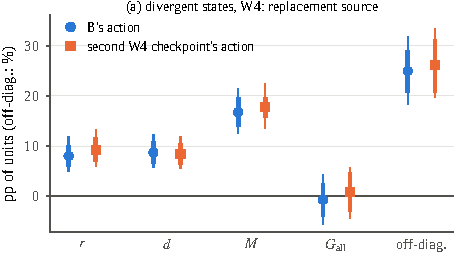
\includegraphics[width=\columnwidth]{figures/f6a_sameprec_rates.pdf}
\end{minipage}\hfill
\begin{minipage}[t]{\columnwidth}
\centering
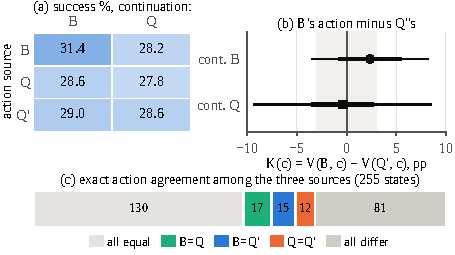
\includegraphics[width=\columnwidth]{figures/f8_commonstate.pdf}
\end{minipage}
\caption{Does an upgrade need a higher bit width? (a)~Each design at its own first divergence, W4 (q4 and q8 GPTQ-W4 pooled; 1020 units; $n_{\mathrm{blk}}=6$): replacing Q's action with B's (circles) or with a second W4 checkpoint's (squares); rescues $r$, damages $d$, turnover $M$ and net $\Gall$ in pp of units, off-diagonal share in \% of divergent states; thick: fixed-pool 95\% ($t$ over block means), thin: new-task 95\% (crossed). (b--d)~Common states (q8; 510 ordinary states, 6 blocks: pre-registered at 3, extended by amendment after the first look): (b)~success (\%) by action source and continuation; (c)~$K(c)$, B's action value beyond a second W4 checkpoint's; here, unlike (a), thick: task-cluster bootstrap 95\%, thin: $t$ (block means) 95\%; shaded: $\pm$3\pp{}; (d)~exact agreement of the three actions. Overlap of affected units, equivalence tests, per-model numbers and two-look intervals: below and Table~\ref{tab:refsfull}.} % src: analysis/fork/out/sameprec_20261004T070601Z.json; analysis/fork/out/sameprec_20261004T070601Z.md (analysis set K = 6); analysis/fork/out/commonstate_q8ext_20261003T231159Z.json; analysis/fork/out/commonstate_q8ext_20261003T231159Z.md; paper/latex/figures/provenance.json (f6a_sameprec_rates, f8_commonstate)
\label{fig:sameprec}
\label{fig:commonstate}
\end{figure*}

% ======================================================================
% FROM: sections/appendix_fidelity.tex (block starting 'The \emph{three-option menu oracle} $E[\max(G,H,F,0)]$ is th', 2 lines)
% WHY: Hindsight three-option menu oracle on Bank P states: not used by the main text, which compares the frozen trigger only with the matched action-replacement oracle.
% ======================================================================
The \emph{three-option menu oracle} $E[\max(G,H,F,0)]$ is the share of states where some arm beats QQ. On Bank P divergent states it is 0.202 over the four W4 cells (state-weighted, the one exception to the paper's equal-weight pools) against 0.117 for the action alone (1127 vs.\ 654 of 5576 states), and 0.191 vs.\ 0.113 over the six core cells. It is hindsight selection that also allows different replacement types, with different costs, so it is not a same-cost deployment comparison and not comparable with the action rule. % src: analysis/fork/out/oracle_trigger_20261002T024423Z.md (§1b)


% ======================================================================
% FROM: sections/appendix_scope.tex (block starting '(sentence inside Table tab:taxonomy caption)', 1 lines)
% WHY: Historical block-f01-only counts from an earlier correction round; superseded by the f01--f03 counts in the same table.
% ======================================================================
% In block f01 alone the corresponding counts were 39 of 56 flips in class (ii), with rates .126/.109/.200 for (ii)/(iii)/(iv); the 58 f01 flips scored in Appendix~\ref{app:token} include the two duplicated U2Q rows. % src: analysis/fork/out/bank_u_f01_20261001T134456Z.md; docs/REPORT_GPT61_20261001_0915.md (correction 1: 39/56 after deduplication)


% (Appendix G follow-ups block restored to the submission appendix by the lead, 2026-10-05: GPT 10-05 ruling keeps label transfer and takeover duration in the appendix.)
